\documentclass[11pt,a4paper]{article}
\usepackage[a4paper,left=22mm,right=22mm,top=20mm,bottom=21mm]{geometry}
\usepackage{fontspec}
\setmainfont{Times New Roman}
\setsansfont{Arial}
\setmonofont[Scale=0.87]{Consolas}
\usepackage[russian]{babel}
\usepackage{amsmath,amssymb,mathtools}
\usepackage{graphicx,booktabs,tabularx,array}
\usepackage{float}
\usepackage{enumitem}
\usepackage{microtype}
\usepackage{xcolor}
\usepackage{caption}
\usepackage{needspace}
\usepackage[unicode,colorlinks=true,linkcolor=blue!45!black,urlcolor=blue!45!black]{hyperref}
\graphicspath{{../figures/}}
\setlength{\parindent}{1.2em}
\setlength{\parskip}{3pt}
\setlength{\emergencystretch}{2em}
\setlist{nosep,leftmargin=1.7em,topsep=4pt}
\captionsetup{font=small,labelfont=bf}
\newcommand{\code}[1]{\texttt{\detokenize{#1}}}
\newcommand{\R}{\mathbb{R}}
\newcommand{\E}{\mathcal{E}}
\newcommand{\N}{\mathcal{N}}
\DeclareMathOperator{\MSE}{MSE}
\DeclareMathOperator{\Std}{Std}
\DeclareMathOperator{\sign}{sign}
\DeclareMathOperator{\clip}{clip}
\newcommand{\titleblock}[2]{\begin{center}{\Large\bfseries #1\par}\vspace{5pt}{\normalsize #2\par}\end{center}\vspace{4pt}}

\begin{document}
\titleblock{Восстановление графа пикселей MNIST}{Протокол и результаты восстановления активной части решётки}

\noindent\textbf{Предмет проверки.}
По изображениям с одинаково перемешанными пикселями строится общий граф признаков.
Оцениваются два свойства: совпадение с исходным соседством пикселей и качество
классификации при подстановке найденного графа в уже обученную нейросеть.
Ни координаты, ни метки цифр не используются при восстановлении.
\par В трёх сохранённых прогонах выбраны 487 активных пикселей и
$1037\pm8$ рёбер. Геометрический F1 равен $0.759\pm0.005$.
При замене эталонного графа восстановленным среднее снижение accuracy составляет
0.51 процентного пункта для GCN и 1.16 пункта для варианта GraphSAGE.
Эксперимент показал успешное приближённое восстановление активной части решётки:
найдено в среднем 80.5\% её рёбер при precision 71.7\%.

\section{Как получен вход алгоритма}
Использован датасет MNIST~\cite{mnist}: 60\,000 обучающих и 10\,000 тестовых
изображений размера $28\times28$ с метками $0,\ldots,9$.
Яркости делятся на 255, каждое изображение представляется строкой из 784 значений.
Для одного запуска генерируется перестановка $\pi$, общая для всех изображений:
\begin{equation}
 X^\pi_{s,j}=X_{s,\pi(j)}.
\end{equation}
Индекс $j$ --- новая позиция, $\pi(j)$ --- исходный пиксель.
Рёбра в новых индексах переводятся для оценки в пары $(\pi(i),\pi(j))$.
Известная оценщику решётка соединяет вертикальных и горизонтальных соседей;
диагоналей и петель в эталоне нет. Она содержит
\begin{equation}
 |E_{\rm grid}|=2\cdot28\cdot27=1512
\end{equation}
рёбер. В алгоритм эта матрица не передаётся.

\section{Разбиение, параметры и выбор графа}
Используются последовательные диапазоны исходного train-архива; предварительного
случайного разбиения изображений нет. Границы ниже --- индексы Python с исключённым правым концом.
\begin{center}\small
\begin{tabularx}{\linewidth}{@{}l r X@{}}\toprule
Назначение & Строки train & Использование\\\midrule
Structure-train & $[0,10000)$ & Активность, корреляции, Lasso, Ridge\\
Structure-validation & $[10000,12000)$ & Энергия, отжиг, выбор штрафа\\
Classifier-train & $[12000,22000)$ & Обучение GNN по меткам\\
Classifier-validation & $[22000,24000)$ & Выбор checkpoint по cross-entropy\\
Official test & все 10\,000 & Итоговая классификация\\\bottomrule
\end{tabularx}\end{center}
Остальные 36\,000 train-изображений в этих повторных прогонах не используются.
Сохранены три seed перестановки: 20260904, 20260917, 20261003.
Соответствующие seed восстановления --- 42, 43, 44; обучения GNN --- 100, 101, 102.
Разбиения изображений одинаковы; между запусками меняются перестановка признаков
и случайные состояния восстановления и обучения.
\par Восстановление использует $B=4$, $K=24$, Ridge $\alpha=0.01$,
2000 шагов отжига и 12 предложений на шаг. Для каждого запуска независимо строятся
три графа при $\lambda\in\{0.08,0.10,0.12\}$.
Сравнивается непенализированная сумма логарифмов проверочных ошибок:
\begin{equation}
 L_\lambda=\E_\lambda(G_\lambda)-2\lambda|E_\lambda|,\qquad
 L_*=\min_\lambda L_\lambda.
\end{equation}
Из графов с $L_\lambda\le L_*+0.01|L_*|$ выбирается самый разреженный.
Во всех трёх опытах из проверенной сетки выбран штраф $0.08$.

\clearpage
\section{Сравниваемые графы}
\begin{description}[leftmargin=0pt,itemindent=0pt]
\item[Эталонная решётка.] $A_{\rm ref,ij}=A_{\rm grid,\pi(i),\pi(j)}$.
Известна оценщику и используется при обучении GNN. В старых JSON называется Oracle.
\item[Восстановленный граф.] Выход процедуры Lasso, Ridge-энергии, pruning и отжига.
Размер графа определяется выбранной конфигурацией и данными.
\item[Correlation top-$E$.] Среди тех же активных вершин выбираются $|E_{\rm rec}|$
пар с наибольшей \emph{обычной абсолютной корреляцией Пирсона} на structure-train.
Блочный score из алгоритма здесь не используется. Активное множество и бюджет рёбер
передаются из результата восстановления.
\item[Случайный граф.] Равномерный выбор без возвращения $|E_{\rm rec}|$ пар активных вершин.
Совпадает число рёбер; распределение степеней не сохраняется.
Имя \code{Random degree-matched} в старых GNN-метриках ошибочно; корректное название --- edge-matched.
\item[Неверно сопоставленная решётка.] Вход остаётся $X^\pi$, но используется
$A_{\rm grid}$ без согласованной перестановки. В ней 1512 рёбер.
\end{description}

\section{Что именно делает классификатор}
Использованы небольшие собственные реализации на PyTorch, основанные на идеях
GCN и GraphSAGE~\cite{gcn,sage}. Применённые варианты архитектур заданы формулами ниже.
Скрытая размерность --- 12, выход --- 10 классов; обучение выполняется с нуля.
Для GCN используется нормировка
\[
 S=(D+I)^{-1/2}(A+I)(D+I)^{-1/2},
\]
где $D$ --- диагональная матрица степеней $A$.
Для одного изображения $h^{(0)}=x^\pi\in\R^{784\times1}$ код вычисляет
\begin{align}
 h^{(1)}&=\operatorname{ReLU}(h^{(0)}W_1+\mathbf1b_1^\top),\\
 h^{(2)}&=\operatorname{ReLU}(S h^{(1)}W_2+\mathbf1b_2^\top),\\
 \ell&=W_o\operatorname{vec}(S h^{(2)})+b_o.
\end{align}
Для варианта SAGE определим $B=D_*^{-1/2}AD_*^{-1/2}$,
$D_{*,ii}=\max(d_i,1)$; петли не добавляются. Тогда
\begin{align}
 h^{(1)}&=\operatorname{ReLU}([h^{(0)}\Vert Bh^{(0)}]W_1+\mathbf1b_1^\top),\\
 h^{(2)}&=\operatorname{ReLU}([h^{(1)}\Vert Bh^{(1)}]W_2+\mathbf1b_2^\top),\\
 \ell&=W_o\operatorname{vec}(h^{(2)})+b_o.
\end{align}
В варианте GraphSAGE применяется симметричная нормировка соседства.
В обеих моделях признаки всех вершин объединяются операцией \code{flatten}.
Последний линейный слой содержит отдельные веса для каждой позиции.
Порядок вершин фиксирован для всех изображений.
\par Каждый классификатор обучается шесть эпох AdamW: learning rate $0.002$,
weight decay $10^{-4}$, batch size 512. Выбирается checkpoint с минимальной
cross-entropy на classifier-validation. После этого для всех графов выполняется
оценка с одними весами, без шагов оптимизатора. Весь классификационный запуск,
включая обучение на согласованной решётке, уже ведётся в переставленной нумерации.

\clearpage
\section{Визуальная проверка структуры}
\begin{figure}[H]\centering
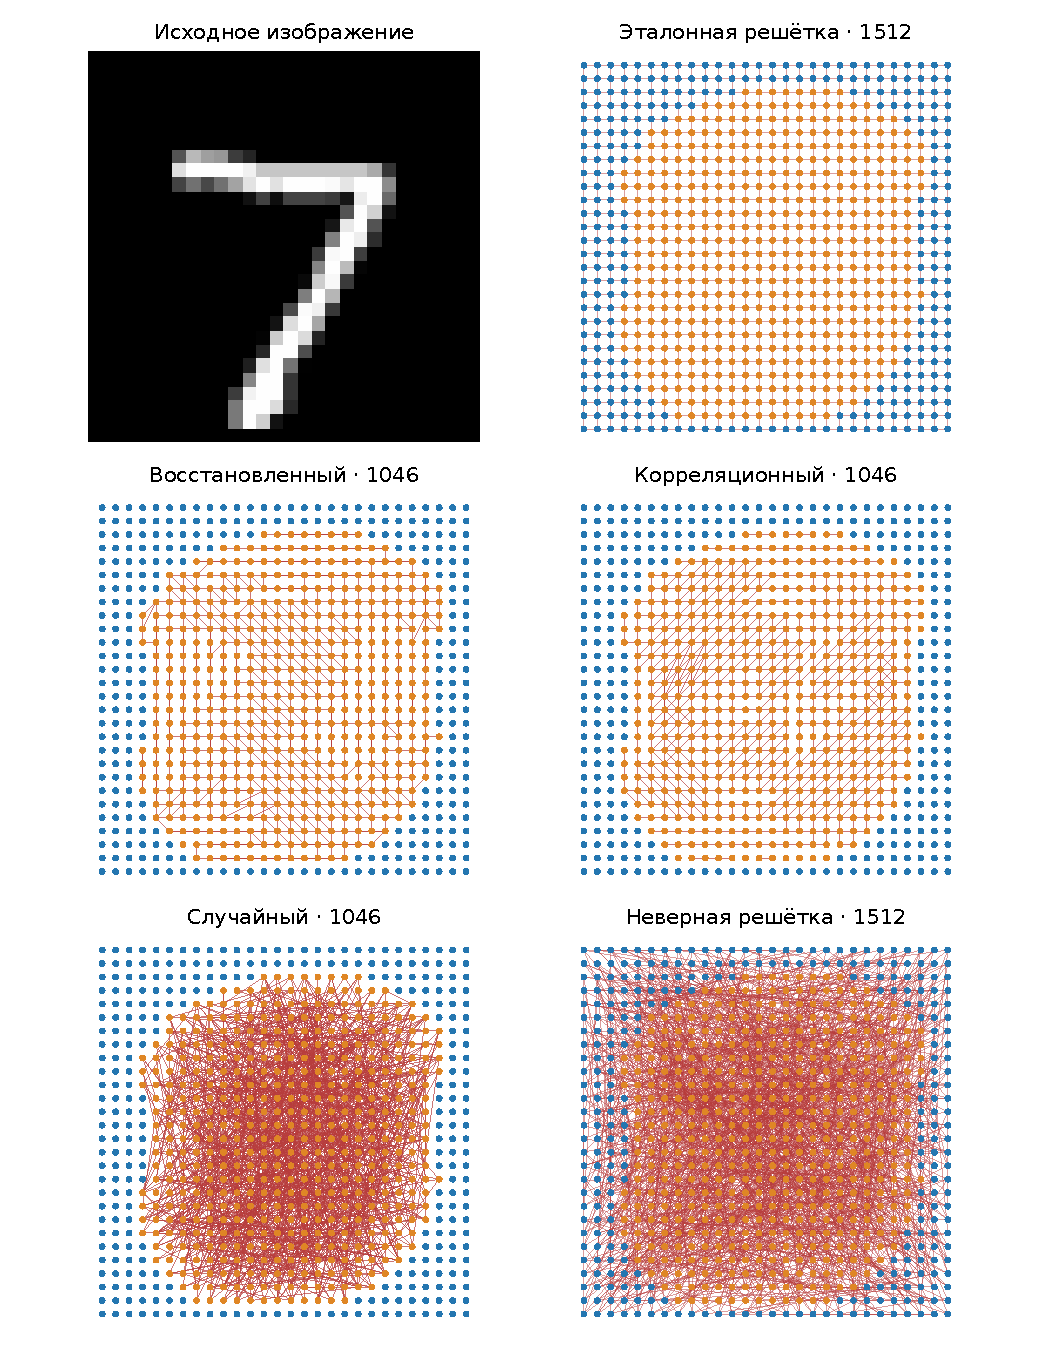
\includegraphics[width=.90\linewidth]{graphs.pdf}
\caption{Первый seed. Оранжевые вершины активны, синие исключены фильтром;
рёбра красные. Исходные координаты используются только при построении рисунка.
Граф восстановления взят из сохранённого NPZ одиночного прогона: его метрики
совпадают с первым повтором. Корреляционный и случайный графы воспроизведены из
сохранённого бюджета и seed; их структурные метрики проверены по JSON.}
\end{figure}

\clearpage
\section{Совпадение с активной частью решётки}
Сравнение проводится с $E_a=\{\{i,j\}\in E_{\rm grid}:i,j\in V_a\}$.
Во всех опытах $|V_a|=487$, неактивных вершин 297, $|E_a|=924$.
Для предсказанного множества $\widehat E$ определяются
\begin{align}
 TP&=|\widehat E\cap E_a|,& FP&=|\widehat E\setminus E_a|,& FN&=|E_a\setminus\widehat E|,\\
 P&=\frac{TP}{TP+FP},& R&=\frac{TP}{TP+FN},& F_1&=\frac{2TP}{2TP+FP+FN}.
\end{align}
Число компонент в таблице относится к индуцированному графу на 487 активных
вершинах. Изолированные 297 неактивных пикселей в него не включаются.
\begin{table}[H]\centering
\small
\caption{Восстановленная структура по каждому seed.}
\begin{tabular}{@{}rrrrrrr@{}}\toprule
Seed & $|E|$ & Precision & Recall & $F_1$ & Компоненты & Макс. размер \\
\midrule
20260904 & 1046 & 0.720 & 0.815 & 0.764 & 4 & 474 \\
20260917 & 1035 & 0.717 & 0.803 & 0.758 & 3 & 482 \\
20261003 & 1030 & 0.716 & 0.798 & 0.754 & 3 & 482 \\
\bottomrule
\end{tabular}
\end{table}

\begin{table}[H]\centering
\small
\caption{Метрики структуры: среднее и выборочное SD.}
\begin{tabular}{@{}lccc@{}}\toprule
Метод & Precision & Recall & $F_1$ \\
\midrule
Восстановленный & $0.717 \pm 0.002$ & $0.805 \pm 0.009$ & $0.759 \pm 0.005$ \\
Correlation top-$E$ & $0.753 \pm 0.003$ & $0.845 \pm 0.003$ & $0.796 \pm 0.001$ \\
Случайный & $0.009 \pm 0.004$ & $0.010 \pm 0.005$ & $0.010 \pm 0.005$ \\
\bottomrule
\end{tabular}
\end{table}

Среднее число рёбер $1037$ на $12.2\%$ больше 924 рёбер активной решётки.
Восстановлено в среднем 80.5\% эталонных связей; 71.7\% найденных рёбер совпадают
с эталоном. Во всех трёх запусках граф содержит 1030--1046 рёбер,
а его крупнейшая компонента охватывает 474--482 из 487 активных вершин.
\par Correlation top-$E$ точнее воспроизводит решётку при переданном бюджете.
Его средний F1 равен 0.796 при том же количестве рёбер, тогда как у полного
алгоритма F1 равен 0.759. Таким образом, найденный алгоритмом бюджет может
использоваться и для корреляционного отбора связей.

\section{Чувствительность к цене ребра}
\begin{table}[H]\centering
\small
\caption{Зависимость размера графа и проверочной ошибки от штрафа.}
\begin{tabular}{@{}rcc@{}}\toprule
$\lambda$ & Рёбра & $L_{\rm val}$ \\
\midrule
0.08 & $1037.0 \pm 8.2$ & $-1071.70 \pm 0.89$ \\
0.1 & $879.0 \pm 9.5$ & $-1039.67 \pm 1.84$ \\
0.12 & $735.3 \pm 2.5$ & $-1004.21 \pm 0.51$ \\
\bottomrule
\end{tabular}
\end{table}

При повышении штрафа число рёбер уменьшается, а $L_{\rm val}$ растёт:
качество линейного предсказания ухудшается. Параметр $\lambda$ позволяет управлять
компромиссом между разреженностью графа и ошибкой предсказания.
Применённое правило выбора конфигурации сохранило вариант со средними 1037 рёбрами.

\clearpage
\section{Результаты классификации с фиксированными весами}
Accuracy --- доля верных классов на 10\,000 test-изображений:
\begin{equation}
 \operatorname{Acc}=\frac1{10000}\sum_s\mathbf1\{\arg\max_c\ell_{s,c}=y_s\}.
\end{equation}
Таблица содержит среднее и выборочное SD по трём запускам.
Парная разность в процентных пунктах вычислена внутри каждого запуска
относительно его эталонного графа, затем усреднена.
\begin{table}[H]\centering
\small
\caption{Test accuracy и парная разность к эталону (п.п.).}
\begin{tabular}{@{}llcc@{}}\toprule
Модель & Граф & Accuracy & $\Delta$ к решётке \\
\midrule
GCN & Решётка & $0.894 \pm 0.012$ & $0.00 \pm 0.00$ \\
GCN & Восстановленный & $0.889 \pm 0.011$ & $-0.51 \pm 0.09$ \\
GCN & Correlation top-$E$ & $0.892 \pm 0.013$ & $-0.23 \pm 0.14$ \\
GCN & Случайный & $0.447 \pm 0.158$ & $-44.73 \pm 17.04$ \\
GCN & Неверная решётка & $0.464 \pm 0.062$ & $-43.03 \pm 7.18$ \\
GraphSAGE & Решётка & $0.911 \pm 0.002$ & $0.00 \pm 0.00$ \\
GraphSAGE & Восстановленный & $0.900 \pm 0.007$ & $-1.16 \pm 0.74$ \\
GraphSAGE & Correlation top-$E$ & $0.898 \pm 0.011$ & $-1.33 \pm 0.99$ \\
GraphSAGE & Случайный & $0.657 \pm 0.139$ & $-25.43 \pm 14.13$ \\
GraphSAGE & Неверная решётка & $0.726 \pm 0.047$ & $-18.50 \pm 4.86$ \\
\bottomrule
\end{tabular}
\end{table}

Дополнительно JSON сохраняет macro-F1 и NLL. Формулы и числа Ridge-energy
к ним не относятся: Ridge используется для восстановления, cross-entropy --- для обучения GNN.
\begin{figure}[H]\centering
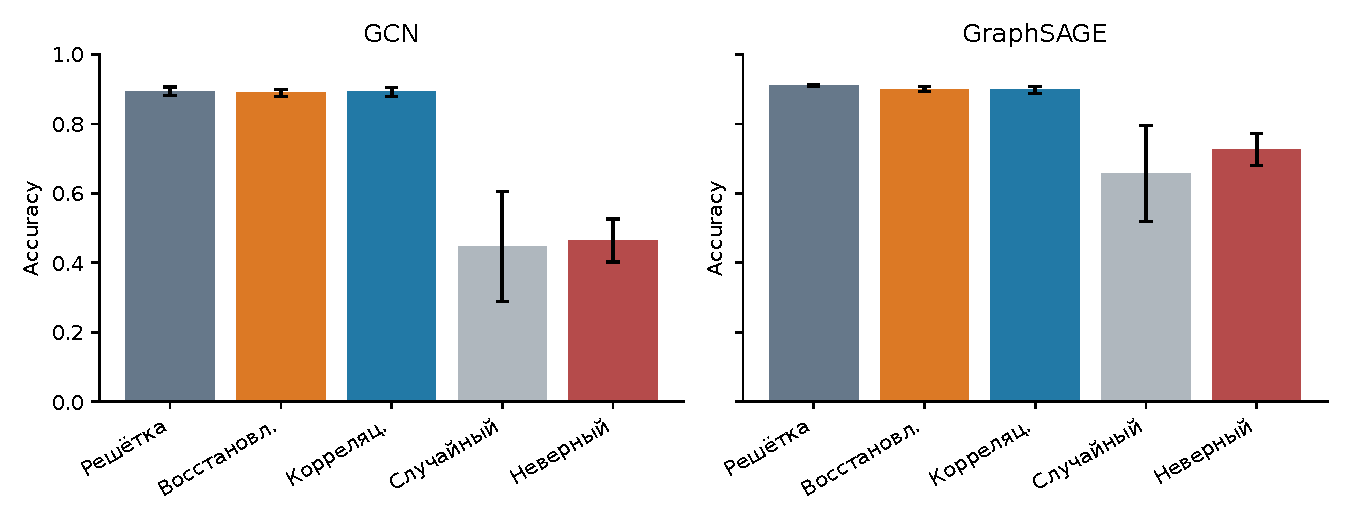
\includegraphics[width=\linewidth]{performance.pdf}
\caption{Accuracy замороженных классификаторов. Полосы обозначают выборочное
стандартное отклонение по трём запускам, а не доверительные интервалы.}
\end{figure}

\clearpage
\section{Основные результаты}
По матрице изображений с неизвестной алгоритму перестановкой пикселей успешно
восстановлено приближённое соседство активной части решётки MNIST.
Координаты, метки классов, исходный граф и его число рёбер для восстановления не использовались.
\begin{enumerate}
\item Выделены 487 активных вершин; почти постоянные пиксели оставлены изолированными.
\item В трёх запусках получены близкие по размеру разреженные графы:
$1037\pm8$ рёбер, precision $0.717\pm0.002$, recall $0.805\pm0.009$,
F1 $0.759\pm0.005$.
\item Размер восстановленного графа превышает размер активной решётки на 12.2\%;
основная часть активных вершин объединена в одну компоненту.
\item При подстановке найденного графа в замороженные классификаторы получены
accuracy $0.889\pm0.011$ для GCN и $0.900\pm0.007$ для варианта GraphSAGE.
Среднее снижение относительно эталонной решётки составило 0.51 и 1.16 процентного пункта.
\item Найденный бюджет рёбер также применён к корреляционному отбору,
который получил геометрический F1 $0.796\pm0.001$.
\end{enumerate}
Основной результат --- восстановление большей части локального соседства пикселей
из одних наблюдений при сохранении разреженной структуры. Повторные запуски дали
близкие значения числа рёбер и качества восстановления.

\section{Исходники и воспроизведение}
Числа этого документа заново рассчитаны из исторического \code{repeated_metrics.json};
обучение ради переоформления отчёта не повторялось.
Исторический \code{pilot_graph.npz} содержит граф и перестановку первого seed.
Для остальных исторических seed сохранены метрики, но не списки рёбер и не веса GNN.
Датасет и сырые артефакты не включены в Git-версию; для сборки PDF достаточно
сохранённых LaTeX-таблиц и векторных рисунков. Для повторного запуска нужен внешний архив MNIST.
\par \code{original_sources/} содержит побайтовый снимок исходников проекта на дату
подготовки пакета. В \code{src/} --- отформатированная копия ядра и переносимый запуск:
\begin{quote}\ttfamily python src/run\_mnist.py --zip PATH\_TO\_MNIST.zip\end{quote}
Он записывает новые метрики и графы в \code{reruns/}, не меняя сохранённые данные отчёта.
\code{--smoke} проверяет выполнение на малой выборке и не воспроизводит исследовательские числа.
Текущий recovery дополнен обработкой неопределённых корреляций и диагностикой стадий;
точная версия до этих дополнений в проекте не сохранена.
Версии зависимостей и инструкции сборки LaTeX приведены в README пакета.

\begin{thebibliography}{9}\small
\bibitem{gcn} Kipf T. N., Welling M. Semi-Supervised Classification with Graph Convolutional Networks.
ICLR, 2017. \url{https://arxiv.org/abs/1609.02907}.
\bibitem{sage} Hamilton W. L., Ying R., Leskovec J. Inductive Representation Learning on Large Graphs.
NeurIPS, 2017. \url{https://arxiv.org/abs/1706.02216}.
\bibitem{mnist} MNIST: описание датасета и официальных размеров разбиений.
\url{https://www.tensorflow.org/datasets/catalog/mnist}.
\end{thebibliography}
\end{document}
